\documentclass[11pt]{article}
\usepackage[utf8]{inputenc}
\usepackage{amsmath}
\usepackage{amsfonts}
\usepackage{amssymb}
\usepackage{tikz}
\usepackage{pgfplots}
\pgfplotsset{compat=1.3}
\begin{document}



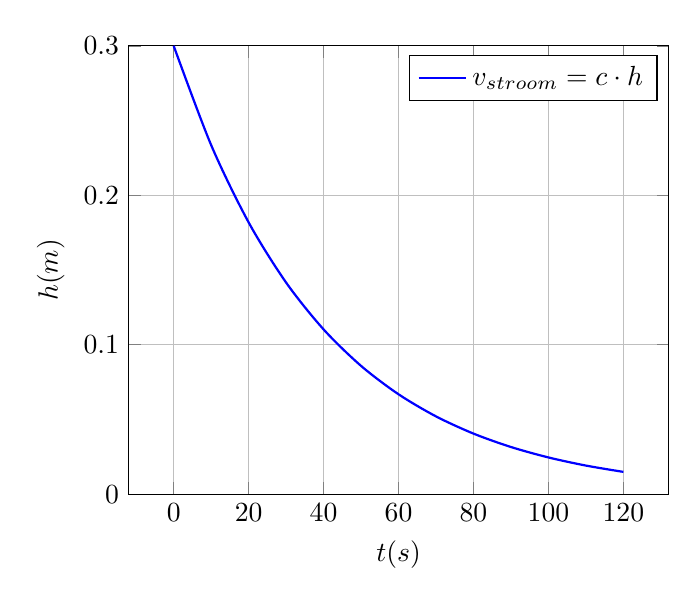
\begin{tikzpicture}
\begin{axis}[
    xlabel = $t(s)$,
    ylabel = {$h(m)$},
    ymax=0.3,
    ymin=0,
    grid=both,
]
%Below the red parabola is defined
\addplot [smooth,
    domain=0:120, 
    samples=100, 
    thick,
    color=blue,
]
coordinates {(0,0.30)(10,0.233567)(20,0.181845)(30,0.141577)(40,0.110226)(50,0.085817)(60,0.066813)(70,0.052018)(80,0.040499)(90,0.031531)(100,0.024549)(110,0.019112)(120,0.01488)};
\addlegendentry{$v_{stroom}=c \cdot h$}
\end{axis}
\end{tikzpicture}

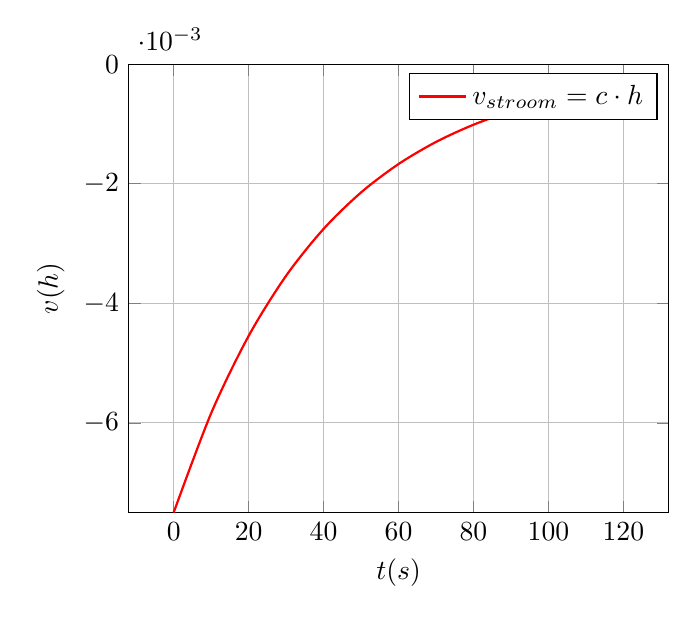
\begin{tikzpicture}
\begin{axis}[
    xlabel = $t(s)$,
    ylabel = {$v(h)$},
    ymax=0,
    ymin=-0.0075,	
    grid=both,
    anchor=north,
]
%Below the red parabola is defined
\addplot [smooth,
    domain=0:120, 
    samples=50, 
    thick,
    color=red,
]
coordinates {(0,-0.0075)(10,-0.005839178)(20,-0.004546133)(30,-0.003539424)(40,-0.002755643)(50,-0.002145426)(60,-0.001670336)(70,-0.001300452)(80,-0.001012476)(90,-0.00078827
)(100,-0.000613713)(110,-0.000477811)(120,-0.000372003
)};
\addlegendentry{$v_{stroom}=c \cdot h$}
\end{axis}
\end{tikzpicture}



\end{document}